\documentclass{article}
\usepackage[utf8]{inputenc}
\usepackage{natbib}
\usepackage{url}
\usepackage{amsmath}
\usepackage{amssymb}
\usepackage{graphicx}
\usepackage{float}
\graphicspath{ { ./images/ } }
\usepackage{hyperref}
\hypersetup{
    colorlinks=false,
    linktoc=all
}
\bibliographystyle{agsm}
\title{Classification of Population Activity in Parkinson's Disease}
\author{Gustav Röhss, Míriam Vall}
\date{VT 2020}
\begin{document}
\maketitle

\section*{Abstract}
\section*{Sammanfattning}

\newpage
\tableofcontents

\newpage
\section{Introduction}

\subsection{Purpose}

\textbf{TODO: Using "brain activity" as supplement for LFP, spiking rates, etc}

The purpose of this project is to attempt to find one or several models for classification of the brain activity in patients with Parkinson's disease.

Furthermore this project aims to, to some extent, use any produced model(s) to evaluate differences is brain activity of different categories.
It is of interest to consider what differences any such model(s) show when comparing brain activity from different brain regions.
It is also of interest to make a similar comparison for the brain activity in different patients.

\subsection{Delimitations}
The authors of this report are not well educated or experienced in studying brain activity.
The model(s) produced are mainly means to serve as a strong foundation for further research into deeper understanding of Parkinson's disease.
The authors attempt to describe and interpret output produced by the model(s), but do so outside of any broader implications the model(s) show in the further study of Parkinson's disease.

No software used, or produced, both by others and by the authors, is subject to extensive formal verification within the scope of this project. 
The same is true for the datasets used within the scope of this project.
The datasets used are instead assumed to have been produced/recorded to a satisfactory quality for their uses within the scope of this project.

\subsection{Research questions}
\begin{itemize}
    \item How can effective models for classification of brain activity in patients with Parkinson's disease be produced?
    \item How can such models be used to distinguish between brain activity from different regions of brains in patients with Parkinson's disease?
    \item How can such models be used to distinguish between brain activity from different patients with Parkinson's disease?
\end{itemize}

\newpage
\section{Background}

\subsection{Discrete Fourier transform}
The Fourier transform, or more specifically, the family of Fourier transforms, are mathematical tools with a long and rich history and many use cases. 
The Discrete Fourier Transform (DFT) is the version of the Fourier Transform used on discrete points of data (rather than e.g. a continuous function). 
One use case of the Fourier transform is to transform a function of time into a function of frequency. 
The DFT can be said to convert data from the \textit{temporal} (time) domain to the \textit{spectral} (frequency) domain.

Specifically, the Fourier transform can be used to approximately decompose a function, or a series, into a large number of waves of different frequencies and amplitudes. 
This method can be used to approximate the amplitude or power of activity in specific frequencies in a signal made up of waves of many frequencies \citep{Fourier}.

\textit{NumPy}, a software library, provides useful tools for usage of the DFT in its' \texttt{fft} package, specifically the \texttt{numpy.fft.fft} (\texttt{FFT}) function \citep{numpy}.

\texttt{FFT} can also be given input to pad the input array with additional zeroes. 
The user then receives a \textit{higher fidelity} output; output information for a larger amount of frequencies.
This can be shown by the \texttt{FFT}-helper function, \texttt{numpy.fft.fftfreq} (\texttt{FFTFREQ}). 
The \texttt{FFTFREQ} function takes arguments \textit{window length} and \textit{sample spacing}, and returns an array of \textit{unit frequency bin centers}. 

The amplitude spectrum for \texttt{FFT} output is obtained by taking the absolute values of the output from the \texttt{FFT} complex-valued output array, specifically using the \texttt{numpy.abs} (\texttt{ABS}) function \citep{numpy}.

\subsection{k-Means}
The k-Means algorithm is a clustering algorithm. 
One noticeable peculiarity of the k-Means algorithm is that the user makes a choice of \textit{k}, the amount of clusters. 

The algorithm works by first randomly generating \textit{k} initial \textit{cluster mean vectors}. 
These are vectors with the same dimensionality as the data samples to be clustered. 
The algorithm then attempts to minimize the \textit{within-cluster sum of squares} of samples assigned to each cluster; the sum of square (Euclidean) distances from the cluster mean vectors, taken over the individual data samples.
The algorithm works iteratively. 
\begin{itemize}
    \item Each sample is assigned to the cluster for which the square distance is minimized.
    \item New cluster mean vectors are created from the mean of the new assignments of samples to clusters.
\end{itemize}
The iteration ends when the cluster mean vectors no longer change (possibly within some tolerance), or a set amount of iterations is reached \citep[p258-260]{PractStats}.

The \textit{scikit learn} software library has an implementation of the k-Means algorithm in its' \texttt{sklearn.cluster.KMeans} module \texttt{(KMeans)}, and is the implementation used in this project \citep{SKLEARN}.

\subsection{Principal component analysis}
One method for extracting lower-dimensional features from higher-dimensional data is by using principal component analysis (PCA).
Specifically, PCA refers to the computation and use of principal components (PCs).
For a set of data, a PC is a direction in the space of the data's features along which the data samples are highly variable.
It's possible for a linear combination of PCs to describe all samples in a dataset with a great degree of accuracy.
If the amount of PCs required for this is lower than the amount of features in the data samples, PCA becomes an effective means of feature reduction for that dataset.
The PCs produced can also be used to visualize the data, and the individual components can be interesting for analyzing the data in their own right \citep[p374-380]{ISLR}.

The \textit{scikit learn} software library enables easy computation of PCs using \texttt{sklearn.decomposition.PCA} (\texttt{PCA})
It also allows the user to transform members of a dataset into their respective representation under a certain set of PCs. 
It should be noted that such a representation is often approximate.
Furthermore, the user is able to see the \textit{explained variance} and \textit{ratio of explained variance} for each PC produced for a specific dataset \citep{SKLEARN}.

\newpage
\section{Methods}
Some methods in this project focused on amplitudes of activity in the spectral domain for the data used in the scope of this project.
The reasoning behind this is that previous research on Parkinson's disease has shown that LFP activity in the beta-range is abnormally synchronized compared to that of the same activity in subjects unaffected by Parkinson's disease. \textbf{TODO: Source}
This suggests that such activity might embed additional useful information for research, and possibly a means for classification. 

\subsection{Spectrum feature extraction}
One important method for feature extraction used in this project was the DFT, using \texttt{FFT}. 
The data was first split into uniform-sized (in array length) \textit{epochs}.
Software implemented for this end was designed such that the \textit{epoch size} could be varied.
Each such epoch was then transformed using \texttt{FFT}.

Interpreting \texttt{FFTFREQ} for the data used in this project, it takes input epoch size (in number of points) and time between samples (multiplicative inverse of sampling frequency). 
It returns an \textit{array index-to-frequency in Hertz} mapping for the output of \texttt{FFT} \citep{numpy}.

The \texttt{ABS} function was used to produce the amplitude spectrum of \texttt{FFT} output. 
\texttt{FFTFREQ} was used to find indices in the \texttt{FFT} output representing frequencies in a certain range.
This range was implemented to be variable.

Using this process, for each epoch a \textit{feature vector} was produced. 
Each value in the vector represents an amplitude of LFP activity for a specific frequency, epoch, channel, and session.
For ease of reference, these vectors will be referred to as \textit{spectrum feature vectors} (SFVs) in this report.

\subsection{k-Means as a visualization heuristic}\label{KM Method}
Initially, k-Means was considered as a means for clustering SFVs in an attempt at classification. 
Attempting to support this choice with an argument as to why it is an appropriate choice of algorithm for this particular use case proved difficult.
However, a heuristic argument can be presented.

The SFVs represent a portion of an amplitude spectrum. 
The square of an amplitude spectrum is a power spectrum \citep{numpy}.
The distance between a cluster mean vector (as generated by k-Means) and a SFV can therefor be interpreted as a "difference in amplitude"-spectrum.
As such, the square of this distance can be interpreted as a "difference in power"-spectrum.
Then, when using k-Means with the SFVs, the "distance" the algorithm will be attempting to minimize is the sum of this "difference in power"-spectrum; or just difference in power.

To reiterate, the presented argument should not be considered extensive for this use case, but rather should be considered a heuristic motivation for its' use as, primarily, a method of visualization.

With this in mind, \texttt{KMeans} was used to produce cluster means and assignments for some subsets of SFVs produced.
Specifically, a set of SFVs for all channels of a certain session were first produced.
A subset of these SFVs were then used as training data for \texttt{KMeans}.
The resulting \texttt{KMeans} model was then used to classify (predict) the entire session-SFV-set.
This procedure was repeated for several different sessions.
The parameters used for \textit{k} for \texttt{KMeans}, the epochs size, and the range of frequencies included in the SFVs are able to be varied in order to produce extensive results. 

\subsection{Usage of principal component analysis}\label{PCA Methods}
In order to better describe the SFVs, PCA was used.

The specific PCs of the SFVs are of interest, as they describe the spectrum-components along which LFP activity vary the most.
Analyzing these specific PCs and how they differ for different subsets of SFVs might highlight key similarities and differences in the LFP activity of different brain regions or subjects.

It is also interesting to consider the PCs of the total set of all SFVs produced. 
Should a small amount of PCs prove able to explain a high ratio of variance in the dataset, this would serve as a strong means for feature reduction, which could then be used in further research.
The PCs produced would then also describe in a more easily digestible manner the key spectral components of any LFP activity in this dataset, and have implications for using similar methods for classification of other sets of LFP activity, and possibly brain activity and time-signals in general.
Such a set of PCs could also be used to highlight differences between different LFP categories.
Should the distribution of SFVs transformed into PC representations under this model be considerably different for different brain regions or animals, this would have implications for classification attempts of LFP activity.

The process for producing PCs was straightforward.
Using \texttt{PCA}, either with some subset of available SFVs, or the entire set of SFVs, the PCs for these sets were produced.

\newpage
\section{Results}

\textbf{TODO: Introduction to results.}

\subsection{Spectrum feature vectors}\label{SFV Results}
Produced SFVs can be visualized using the \textit{matplotlib} software library's useful \texttt{matplotlib.pyplot.imshow} (\texttt{IMSHOW}) function \citep{MPL}.

Figure \ref{fig:GP1} and figure \ref{fig:STR2} show SFVs for channels \texttt{gp\_lfp1} and \texttt{str\_lfp10} for sessions \texttt{NPR052e.10} and \texttt{NPR064.b08}, respectively. 
For both figures, each column represents a single SFV. 
For both figures, higher brightness represent higher amplitude of LFP activity in that epoch and frequency.
For both figures, each column is the SFV generated for a specific epoch of activity, displayed chronologically. 
Figure \ref{fig:GP1} shows 780 epochs, and figure \ref{fig:STR2} shows 778 epochs. 
For both of these sessions the sampling frequency is 16 kHz. 
For both of these sets of produced SFVs, the epoch size in amount of data points (sampled at sampling frequency) is 2048, resulting in an epoch size of 128 ms. 
For each of these sets of produced SFVs, there are 46 frequencies sampled. 
Specifically, the input was padded with to a length of 16384 in order to produce a higher fidelity output, and all frequency samples in the ranges of 5 Hz - 50 Hz were selected. 
This results in 46 equally-spaced frequency samples, the lowest being approximately 5.86 Hz and the highest being approximately 49.8 Hz. 
The parameters can be considered arbitrary due to easily being changed.
In this specific configuration, the frequency range was selected to be somewhat wider than the beta-range of frequencies.
The epoch size was chosen to be somewhat longer than the shortest length of a beta-burst \citep{Cagnan}.

These figures are, clearly, a very small subset of the total set of produced SFVs. They also represent only a very small subset of possible configurations of SFVs in regards to epoch size, sampled frequencies, and amount of frequency samples.

\begin{figure}[H]
    \centering
    \centerline{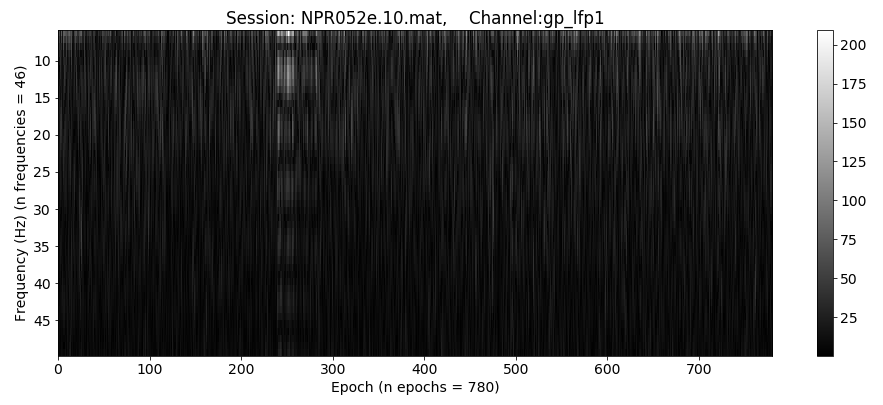
\includegraphics[width=1\textwidth]{images/GP1.png}}
    \caption{SFVs for Globus Pallidus LFP channel of a specific session.}
    \label{fig:GP1}
\end{figure}

\begin{figure}[H]
    \centering
    \centerline{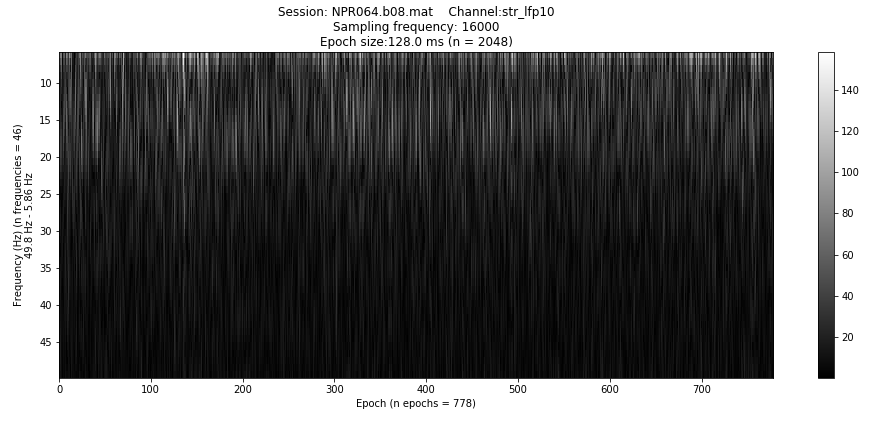
\includegraphics[width=1\textwidth]{images/STR2.png}}
    \caption{SFVs for Striatum LFP channel of a specific session.}
    \label{fig:STR2}
\end{figure}

\subsection{k-Means}

To visualize k-Means predictions for a k-Means model trained on SFVs, \texttt{IMSHOW} was used once more.
Some of the produced figures are figure \ref{fig:KM4} and figure \ref{fig:KM16}.
In order to better relate to the heuristic argument presented in subsection \ref{KM Method}, the colors for class assignments were chosen to be sorted by the "sum of power spectrum" (sum of squares) of the cluster centers.
Lower class index (refer to color bar in either figure) represents lower sum of power spectrum.
The indices of class assignments will be presented as "low" and "high" for brevity.

In the figures, each row represents the class assignments for a specific channel in the set.
The columns represent epochs.
Each colored "slice" is the prediction of a single SFV to a class, the result of a trained \texttt{KMeans} model.
The particular channel names are not shown in these figures, but include both STR and GP channels.
The SFVs are identical in production parameters to those presented in the previous section.

The most important thing to note about these figures is how different channels in the same (or close) epochs tend to be given equal class assignments excessively. 
The authors interpret the class assignments for adjacent epochs to often be "close", meaning that class assignments seem to be followed by slightly higher or slightly lower class assignments, this was however not researched more thoroughly and should be considered an informal observation.
Also of note are "streaks" of higher class assignments for specific channels.
Examples include for channel 4 at about epoch 700, and channel 12 at about epochs 330-420 (rough estimates).
There are also "pillars" of excessively similar assignments for all channels at about epochs 140, 290, and 550 (rough estimates).

\begin{figure}[H]
    \centering
    \centerline{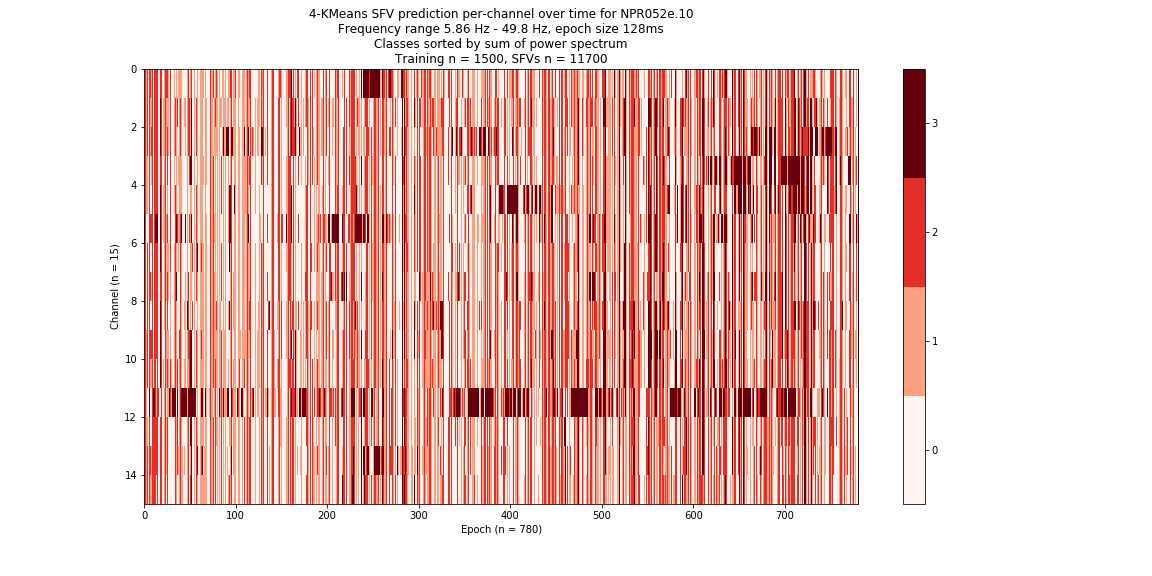
\includegraphics[width=1\textwidth]{images/KM4.png}}
    \caption{4-k-Means of channels for specific session}
    \label{fig:KM4}
\end{figure}

\begin{figure}[H]
    \centering
    \centerline{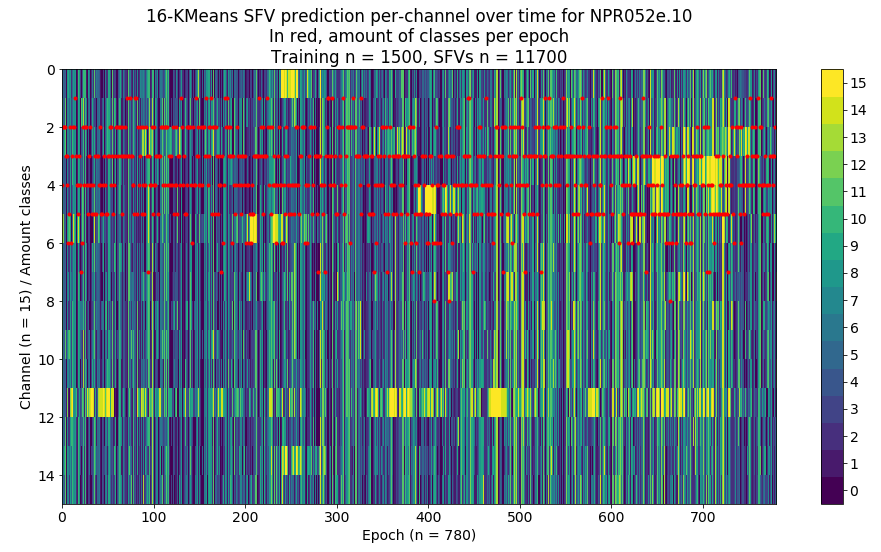
\includegraphics[width=1\textwidth]{images/KM16.png}}
    \caption{16-k-Means of channels for specific session}
    \label{fig:KM16}
\end{figure}

\subsection{Principal component analysis of spectrum feature vectors}

\textbf{TODO: Slightly increase height of PCS plots.}
\textbf{TODO: Crosscorrelations within GP, STR.}

The method outlined in subsection \ref{PCA Methods} was performed using a set of 362,184 SFVs produced with parameters identical to those described in subsection \ref{SFV Results}.
Indeed, the SFVs shown in figures \ref{fig:GP1} and \ref{fig:STR2} are part of the set used to compute the \texttt{PCA} model.

The first thing to consider about the PCs computed for the set of SFVs are the PCs themselves.
Figure \ref{fig:PCS} shows these, as well as their respective explained variance ratios. 
This figure was produced using the \texttt{matplotlib.pyplot.plot} (\texttt{PLOT}) function.
In this specific case, eight PCs were produced, as this was the points where their cumulative sum of explained variance ratio was above 90\%.
These PCs can be interpreted as being parts of which a linear combination approximately describe all of the SFVs from which they were computed.

\begin{figure}[H]
    \centering
    \centerline{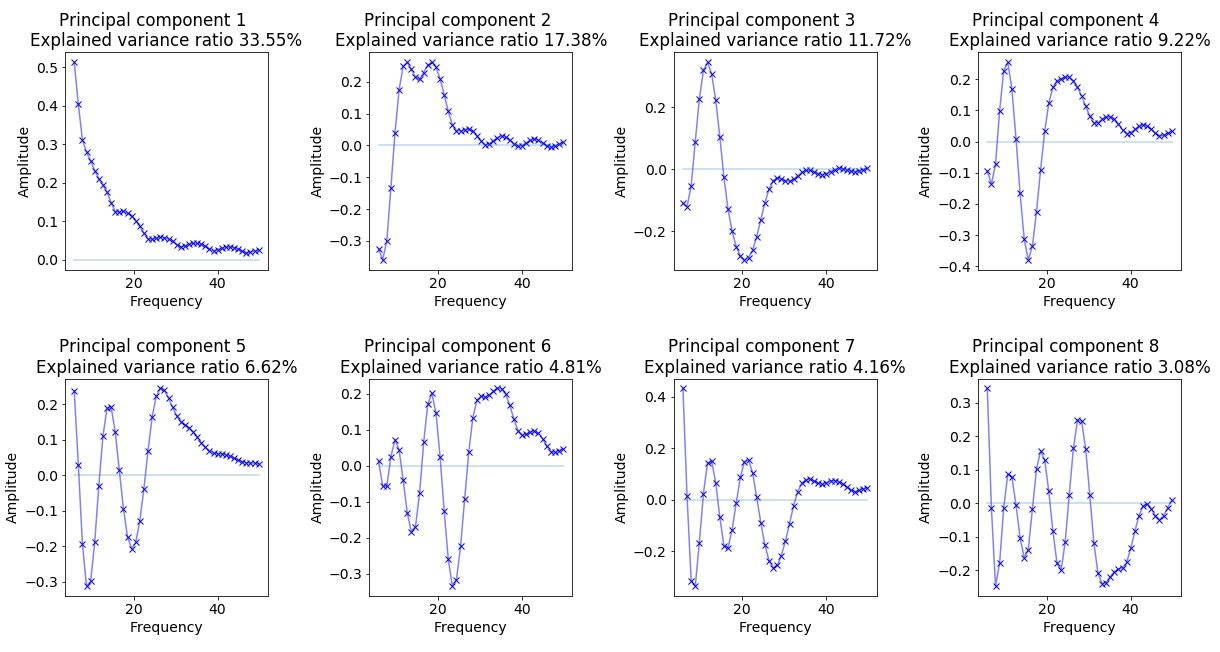
\includegraphics[width=1\textwidth]{images/PCA/PCS.png}}
    \caption{Principal components of SFV-set}
    \label{fig:PCS}
\end{figure}

Having computed these PCs, the approximate probability distributions of the individual components as they appear in the set of \texttt{PCA}-transformed SFVs are shown in figure \ref{fig:PCAPDF}. 
In order to better visualize the long tails of these distributions, the probability distributions of the logarithms (base 2) of the individual components are shown in figure \ref{fig:PCAPDFLG2}.

\begin{figure}[H]
    \centering
    \centerline{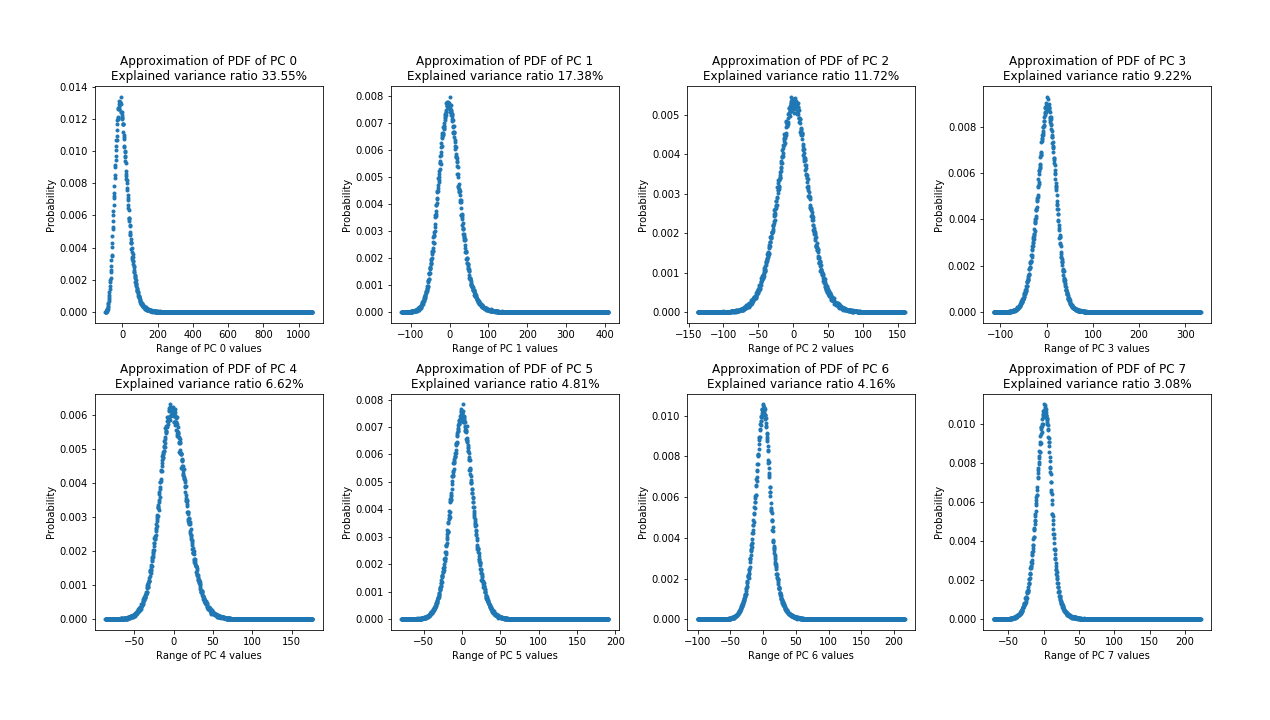
\includegraphics[width=1\textwidth]{images/PCA/PCAPDF.png}}
    \caption{Approximate distributions of principal components of SFV-set}
    \label{fig:PCAPDF}
\end{figure}

\begin{figure}[H]
    \centering
    \centerline{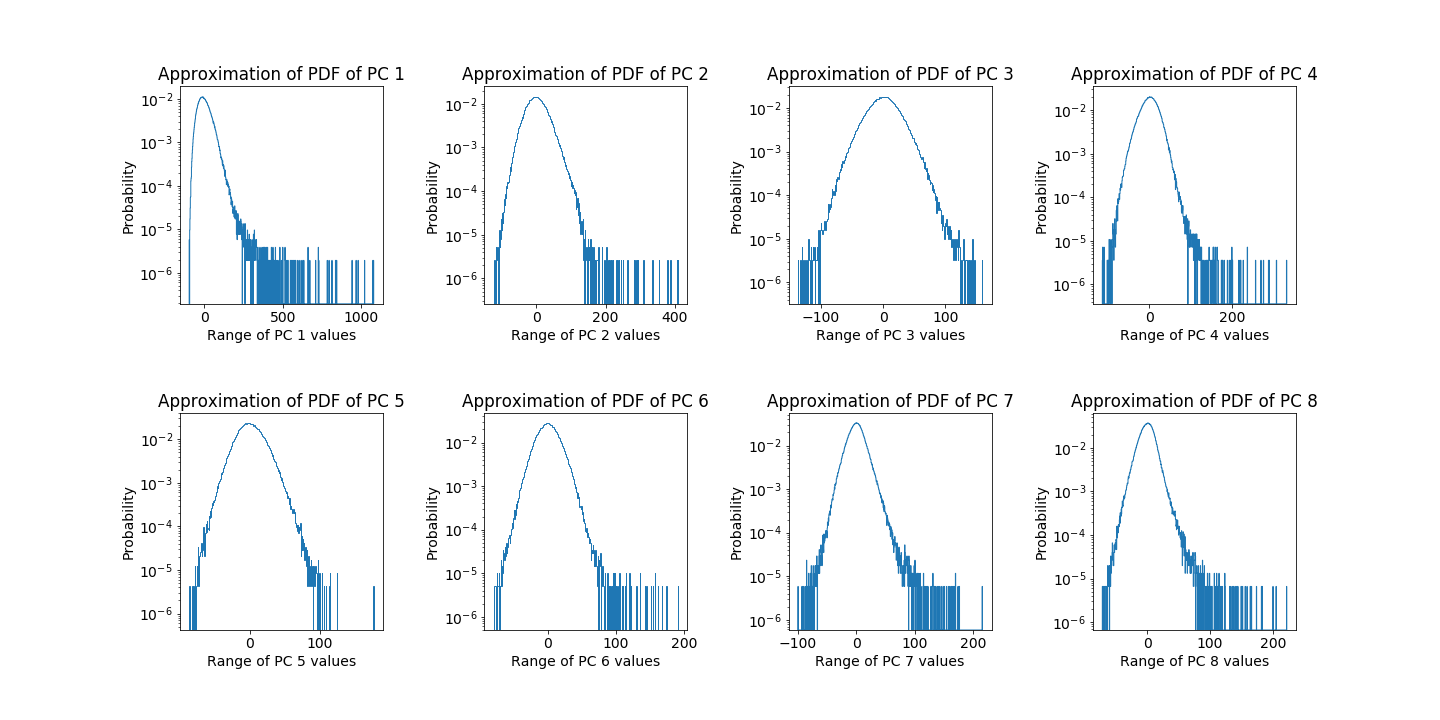
\includegraphics[width=1\textwidth]{images/PCA/PCAPDFLG2.png}}
    \caption{Approximate distributions of \begin{math}log_2\end{math} of principal components of SFV-set}
    \label{fig:PCAPDFLG2}
\end{figure}

The information shown in figures \ref{fig:PCAPDF} and \ref{fig:PCAPDFLG2} is also shown in figures \ref{fig:PCAPDFBOTH} and \ref{fig:PCAPDFBOTHLG2}, except with channels from STR kept separate from those of GP.
Notably, GP exhibits distributions with more width and higher peaks.

\begin{figure}[H]
    \centering
    \centerline{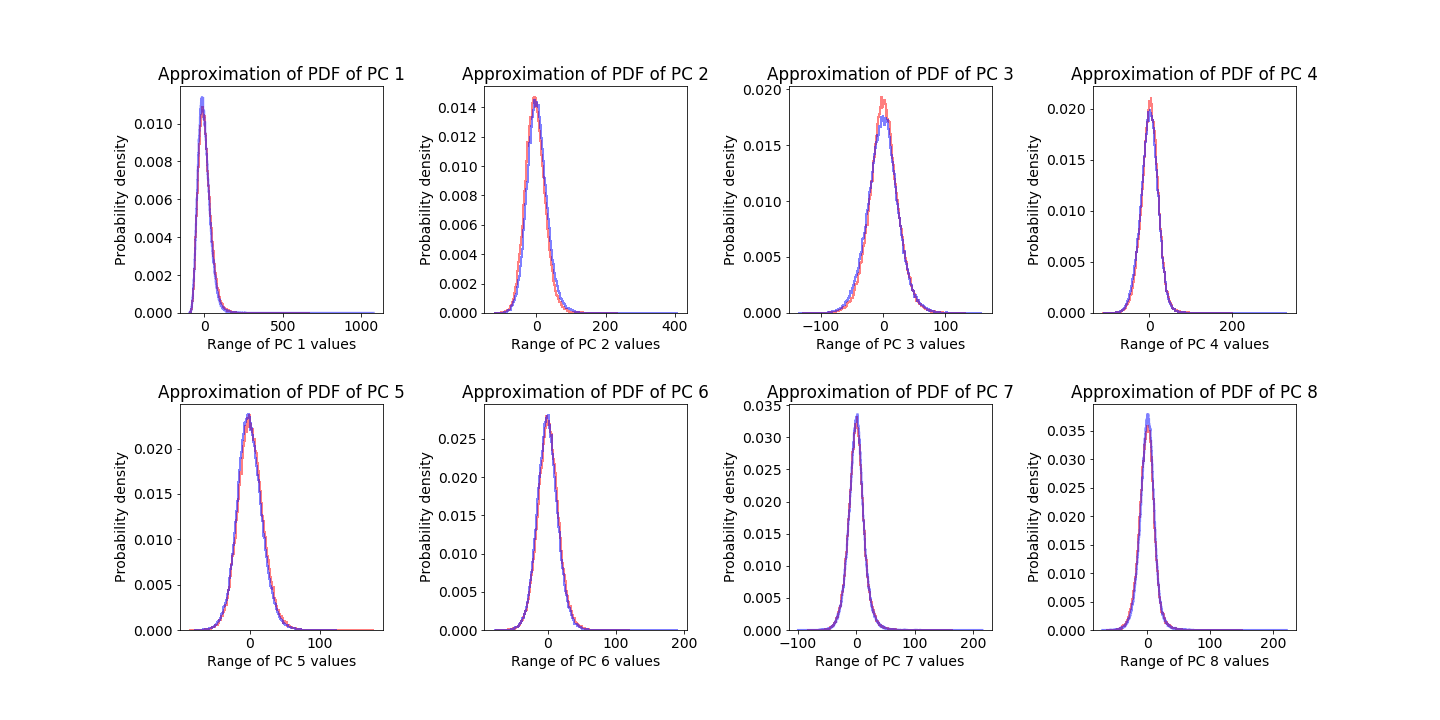
\includegraphics[width=1\textwidth]{images/PCA/PCABOTH.png}}
    \caption{Approximate distributions of principal components of SFV-set, separated by channel type}
    \label{fig:PCAPDFBOTH}
\end{figure}

\begin{figure}[H]
    \centering
    \centerline{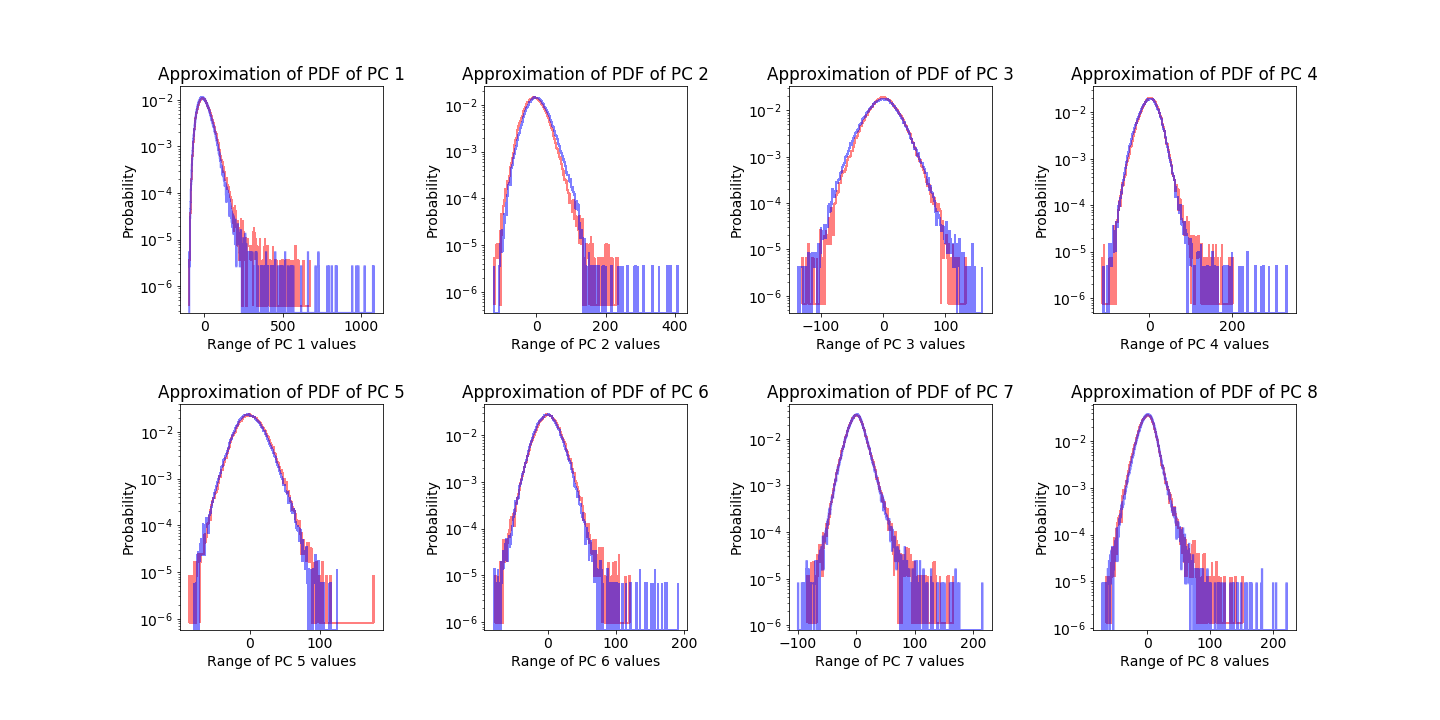
\includegraphics[width=1\textwidth]{images/PCA/PCABOTHLG2.png}}
    \caption{Approximate distributions of \begin{math}log_2\end{math} of principal components of SFV-set, separated by channel type}
    \label{fig:PCAPDFBOTHLG2}
\end{figure}

These figures, of course, don't show how these distributions correlate.
Tables \ref{tab:corrcoefGP} and \ref{tab:corrcoefSTR} show the cross-correlation of \texttt{PCA}-transformed SFVs, for GP and STR channels respectively.
Notably, cross-correlation within STR channels is consistently somewhat low, while it is consistently quite higher within GP channels.

\begin{table}[H]
    \centering
    \begin{tabular}{c|c|c|c|c|c|c|c|c}
          & PC 0 & PC 1 & PC 2 & PC 3  & PC 4 & PC 5 & PC 6 & PC 7  \\
     PC 0 & 1.0  & 0.43 & 0.17 & 0.44  & 0.23 & 0.39 & 0.44 & 0.5  \\
     PC 1 & 0.43 & 1.0  & 0.1  & 0.26  & 0.13 & 0.26 & 0.26 & 0.31 \\
     PC 2 & 0.17 & 0.1  & 1.0  & 0.11  & 0.07 & 0.08 & 0.12 & 0.13 \\
     PC 3 & 0.44 & 0.26 & 0.11 & 1.0   & 0.16 & 0.26 & 0.31 & 0.35 \\
     PC 4 & 0.23 & 0.13 & 0.07 & 0.16  & 1.0  & 0.13 & 0.16 & 0.19 \\
     PC 5 & 0.39 & 0.26 & 0.08 & 0.26  & 0.13 & 1.0  & 0.27 & 0.32 \\
     PC 6 & 0.44 & 0.26 & 0.12 & 0.31  & 0.16 & 0.27 & 1.0  & 0.35 \\
     PC 7 & 0.5  & 0.31 & 0.13 & 0.35  & 0.19 & 0.32 & 0.35 & 1.0  \\
    \end{tabular}
    \caption{Cross-correlation of PCs, GP channels, rounded to two decimals.}
    \label{tab:corrcoefGP}
\end{table}

\begin{table}[H]
    \centering
    \begin{tabular}{c|c|c|c|c|c|c|c|c}
          & PC 0  &  PC 1 &  PC 2 &  PC 3 &  PC 4 &  PC 5 &  PC 6 &  PC 7 \\
     PC 0 &  1.0  & -0.05 &  0.01 &  0.0  &  0.0  & -0.01 & -0.0  &  0.01 \\
     PC 1 & -0.05 &  1.0  &  0.05 &  0.08 &  0.03 &  0.01 &  0.04 &  0.03 \\
     PC 2 &  0.01 &  0.05 &  1.0  &  0.03 & -0.02 &  0.02 &  0.02 & -0.01 \\
     PC 3 &  0.0  &  0.08 &  0.03 &  1.0  & -0.0  &  0.03 & -0.02 &  0.01 \\
     PC 4 &  0.0  &  0.03 & -0.02 & -0.0  &  1.0  &  0.01 &  0.01 & -0.0  \\
     PC 5 & -0.01 &  0.01 &  0.02 &  0.03 &  0.01 &  1.0 &  -0.0  & -0.01 \\
     PC 6 & -0.0  &  0.04 &  0.02 & -0.02 &  0.01 & -0.0 &   1.0  &  0.0  \\
     PC 7 &  0.01 &  0.03 & -0.01 &  0.01 & -0.0  & -0.01 &  0.0  &  1.0  \\
    \end{tabular}
    \caption{Cross-correlation of PCs, STR channels, rounded to two decimals.}
    \label{tab:corrcoefSTR}
\end{table}

\newpage
\section{Discussion}

\newpage
\section{Conclusion}

\newpage
\section{References}
\bibliography{sources}

\end{document}